\documentclass[10pt,a4paper,oneside,fleqn]{report}
\usepackage{geometry}
\geometry{a4paper,left=20mm,right=20mm,top=1cm,bottom=2cm}
\usepackage[utf8]{inputenc}
%\usepackage{ngerman}
\usepackage{amsmath}                % brauche ich um dir Formel zu umrahmen.
\usepackage{amsfonts}                % brauche ich für die Mengensymbole
\usepackage{graphicx}
\setlength{\parindent}{0px}
\setlength{\mathindent}{10mm}
\usepackage{bbold}                    %brauche ich für die doppel Zahlen Darstellung (Einheitsmatrix z.B)
\usepackage[linktocpage={false}]{hyperref}


\usepackage{color}
\usepackage{titlesec} %sudo apt-get install texlive-latex-extra

\definecolor{darkblue}{rgb}{0.1,0.1,0.55}
\definecolor{darkred}{rgb}{0.55,0.2,0.2}

\titleformat{\chapter}[display]{\color{darkred}\normalfont\huge\bfseries}{\chaptertitlename\
\thechapter}{20pt}{\Huge}

\titleformat{\section}{\color{darkblue}\normalfont\Large\bfseries}{\thesection}{1em}{}
\titleformat{\subsection}{\color{darkblue}\normalfont\Large\bfseries}{\thesection}{1em}{}

% Notiz Box
\usepackage{fancybox}
\newcommand{\notiz}[1]{\vspace{5mm}\ovalbox{\begin{minipage}{1\textwidth}#1\end{minipage}}\vspace{5mm}}

\usepackage{cancel}


%\includegraphics[width=0.75\textwidth]{thepic.png}

\begin{document}
\tableofcontents
\setcounter{chapter}{12}
\chapter{Supraleitung}

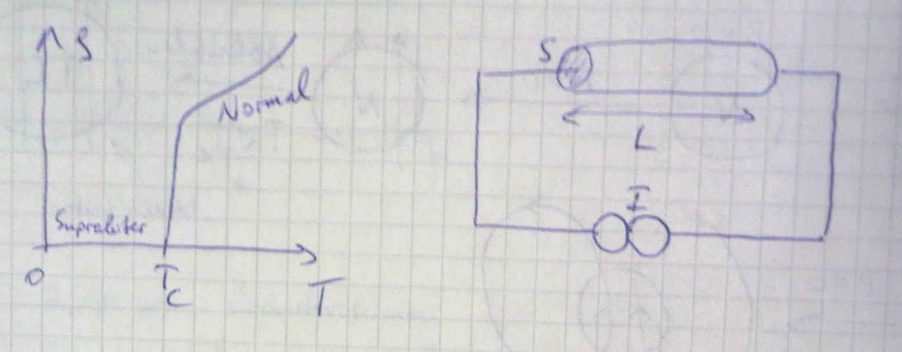
\includegraphics[width=0.75\textwidth]{kap13_01.png}

\[U=RI = \rho\frac{L}{S}I\]

\[\left.\rho\right|_{Cu,T=4,2K}\approx 10^{-9}\Omega m\]

für \(\rho < 10^{-24}\Omega cm\)

1911 Kamerlingli-Onnes

Hg: \(T_c\approx 4K\)

\begin{tabular}{ccc}
  \(N_z\)&\(\rightarrow \)&77K\\
  \(H_z\)&\(\rightarrow \)&20K\\
  \(^4He\)&\(\rightarrow \)&4,2K\\
\end{tabular}

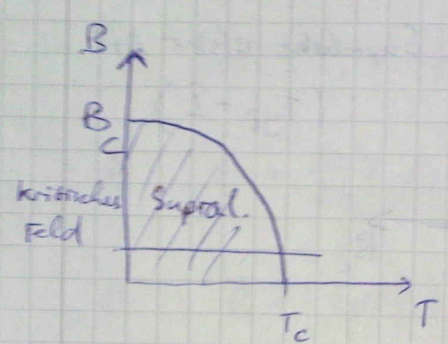
\includegraphics[width=0.45\textwidth]{kap13_02.png}

\begin{tabular}{cc}
  Al&1,2K\\
Im&3,4K\\
Sn&3,7K\\
Pb&7,2K\\
Nb&9,2K\\
--&--\\
NbN&15K\\
\(Nb_3Ge\)&24K\\
1986 \(YBaCu_3O_7\) & 92
\end{tabular}

\(Tl_2Sr_2Ca_2Cu_3O_8 \rightarrow 120K\)

Supralaeiter ist kein 'idealer' Leiter \(\rightarrow \) Meissner-Effekt



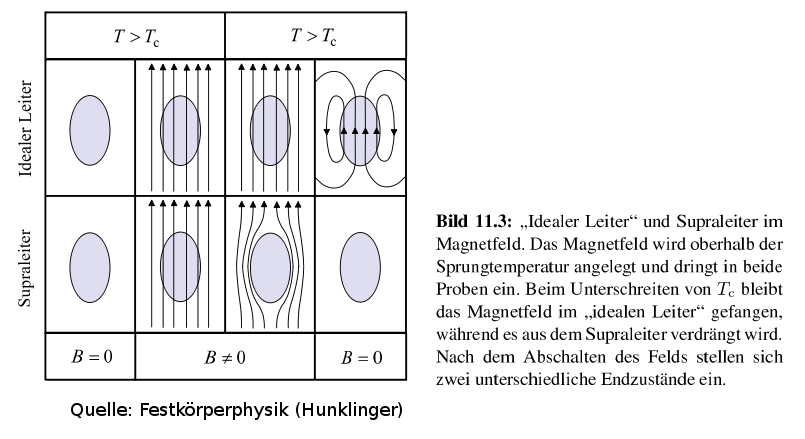
\includegraphics[width=0.75\textwidth]{kap13_03.png}




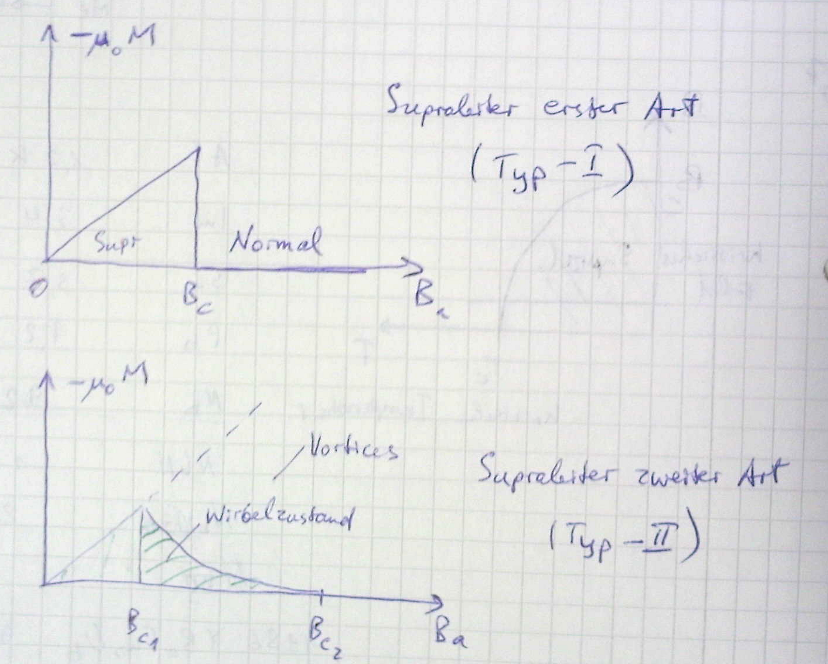
\includegraphics[width=0.75\textwidth]{kap13_04.png}


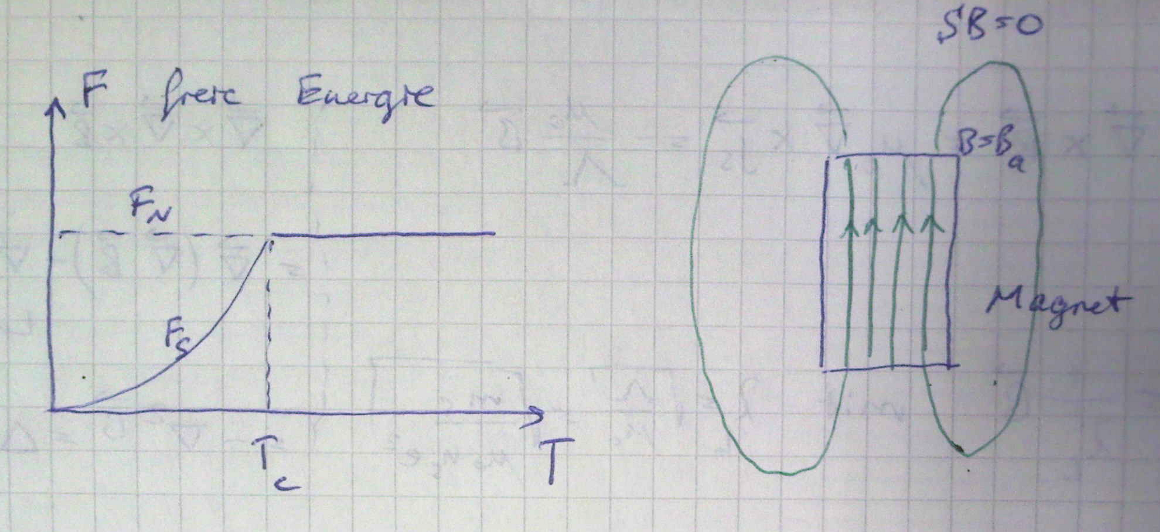
\includegraphics[width=0.75\textwidth]{kap13_05.png}


Arbeit pro Einheitsvolumen der Probe

\[W=-\int_0^{B_a}\vec M\cdot d\vec B_a = \int_0^{B_a} dF_s = \frac{B_a}{\mu_0}dB_a  \]

\[F_S(B_a) - F_S(0) = \frac{B_a^2}{2\mu_0}\]

\section{London-Gleichungen (Postulate)}

\begin{enumerate}
\item[1)] \(\vec E = \frac{\partial}{\partial t}(\Lambda \vec \gamma_S)\) mit \(Lambda = \frac{m_S}{n_Se^2}\)
\item[2)] \(\vec B = -rot(\Lambda \vec j_S)\)
\end{enumerate}

\subsection{Zwei Flüssigkeiten-Modell}

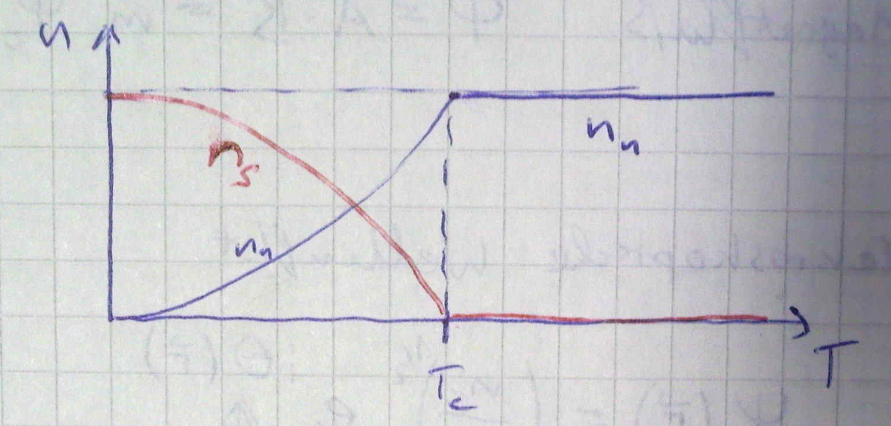
\includegraphics[width=0.75\textwidth]{kap13_06.png}


\[\vec \nabla\times\vec\nabla\times \vec B = \mu_0\vec\nabla\times\vec j_S = -\frac{\mu_0}{\Lambda}\vec B\]

mit \( \vec \nabla\times\vec\nabla\times \vec B = \vec\nabla(\vec \nabla\vec B)-\underbrace{\nabla^2\vec B}_{\text{Laplace}} = -\nabla^2\vec B = \Delta \vec B \)

\[\nabla^2\vec B = \frac{1}{\lambda^2_L}\vec B\]

mit \(\lambda_L = \sqrt{\frac{\Lambda}{\mu_0}} = \sqrt{\frac{m_S}{\mu_0 n_S e^2}}\) als Londonsche eindringtiefe


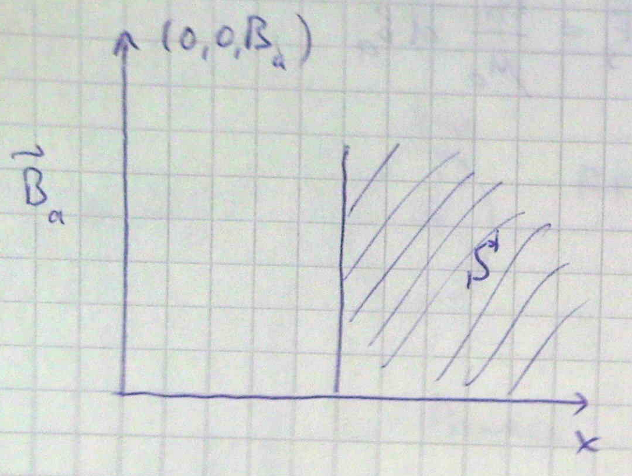
\includegraphics[width=0.75\textwidth]{kap13_07.png}


\[\frac{d^2 B}{dx^2} = \frac{1}{\lambda^2_L}B\]


\[B(x) = B_0e^{-\frac{x}{\lambda_L}}\]


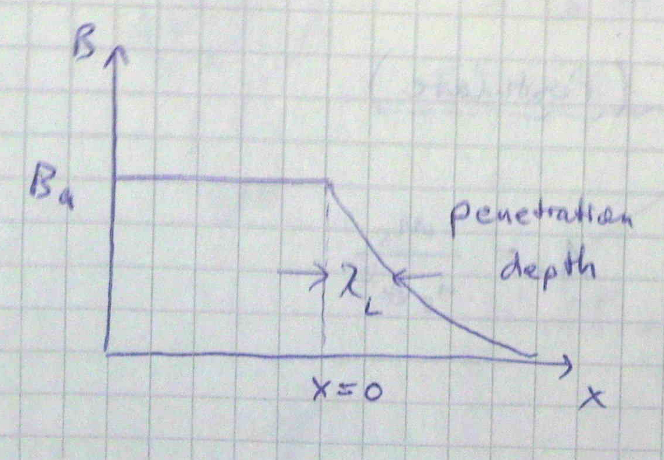
\includegraphics[width=0.75\textwidth]{kap13_08.png}


Für \(B(0) = B_a\), \(B(\infty) = 0\) ergibt sich für \(x>0\):

\[B(x) = B_a e^{-\frac{x}{\lambda_L}}\]


\section{Flußquantisierung}

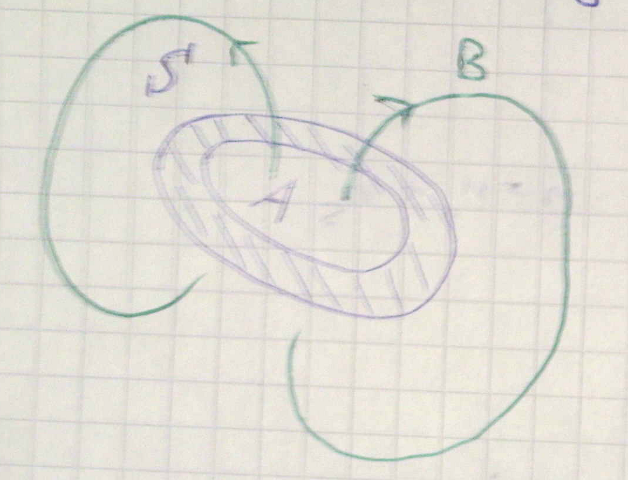
\includegraphics[width=0.45\textwidth]{kap13_09.png}


Magnetfluß \(\Phi = AB = m\Phi_0\), \(\Phi_0 = \frac{h}{2e}=2,7\cdot 10^{-15}V\cdot s\equiv [Wb] \)


Makroskopische Wellenfunktion

\[\Psi(\vec r) \sqrt{\frac{n_S}{2}} e^{i\Theta(\vec r)}\]

Elektronen verhalten sich wie Bosonen-Teilchen


\section{Theorie der Supraleitung}

\begin{enumerate}
\item[1)] 'makroskopische' Theorie GL = Ginszburg-Landau (1956)
\item[2)] mikroskopische Theorie \(\rightarrow \) BSC=Bardeen -Cooper-Schrieffer (1957)
\end{enumerate}

Messung des Isotopeneffekt 

\[T_C\cdot \sqrt{M} = const\] 

mit M Masse der Atome und ist proportional zu \(T_C\propto \omega_D\) der Debye-Frequenz. 

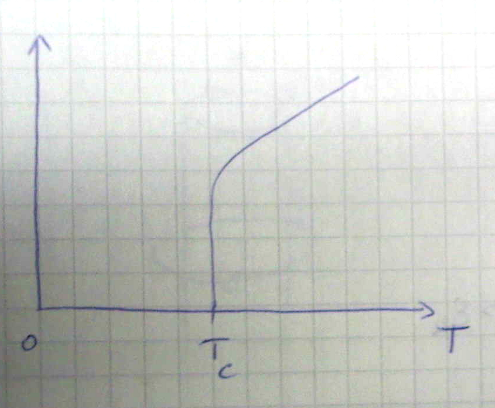
\includegraphics[width=0.45\textwidth]{kap13_10.png}

Wechselwirkung von zwei entgegengesetzen Teilchen, den sogenanten Cooper Paaren:

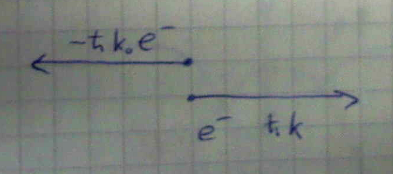
\includegraphics[width=0.45\textwidth]{kap13_11.png}


(1) 'Kielwasser' \(\rightarrow \) eine positive Ladungswolke \(\rightarrow \) anziehen (2)

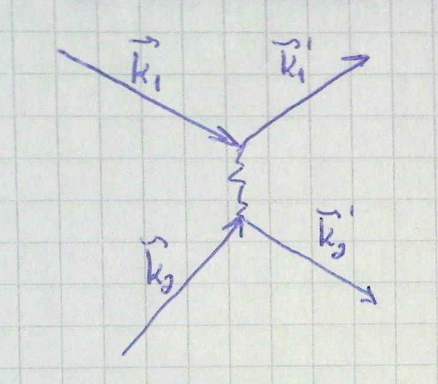
\includegraphics[width=0.45\textwidth]{kap13_12.png}

Die Elektronen \(\vec k_1\) und  \(\vec k_2\) tauschen virtuelle phononen (\(\vec q\)) aus

\[\vec k_1' = \vec k_1-\vec q;\qquad \vec k_2' = \vec k_2-\vec q; \qquad \vec k_1+\vec k_2 = \vec k_1'+\vec k_2' \]

Die Elektronen WW wird durch ein Matrixelement beschrieben:

\[V_{kk'} = \begin{cases}
  -V,|E_k-E_F|\leq\hbar\omega_D  \text{und } |E_k'-E_F|\leq \hbar\omega_D\\
  0, \text{falls nicht der Fall }
\end{cases}\]

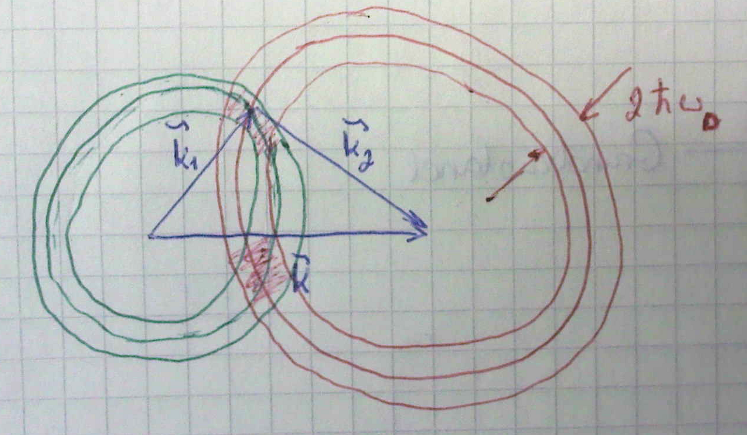
\includegraphics[width=0.45\textwidth]{kap13_13.png}

\[\vec k_1+\vec k_2 = \vec K\]

Im \(\vec k\)-Raum \(\rightarrow \) eine Kugelschale mit der Dicke \(\frac{\Delta k}{k_F}\approx \frac{2\hbar\omega_D}{E_F}\). Phononenauustausch mit gröstmöglicher Wahrscheinlichkeit für \(\vec K =0 \). Entstehung der Cooper-Paare.

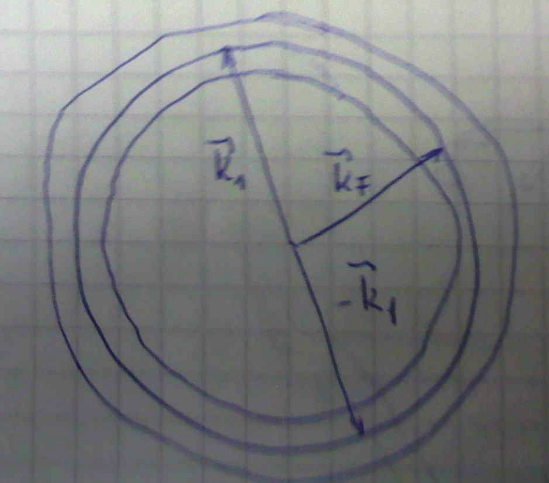
\includegraphics[width=0.45\textwidth]{kap13_14.png}


Zweiteilchen- Wellenfunktion

\[\Psi = A e^{i\vec k_1\vec r_1}\cdot e^{i\vec k_2\vec r_2}   \]

mit \(\vec k_1 = \vec k = -\vec k_2\) und \(\vec r = \vec r_1-\vec r_2\)

\[ \Psi = \sum_k A_k e^{i\vec k\vec r}\]

BCS- Grundzustand:

\[E_{\sum} = \sum \underbrace{2\epsilon_k v_k^2}_{\text{kinetische Energie}}+\sum \underbrace{V_{kk'}v_ku_kv_{k'}u_{k'}}_{\text{Streuung }\rightarrow (k',-k')}\]

mit \(\epsilon_k = \frac{\hbar^2k^2}{2m}-\frac{\hbar^2k^2_F}{2m}\), \(\frac{\hbar^2k^2_F}{2m} = E_F\)

\(v_k^2 =\) die Wahrscheinlichkeit dass der Zustand \((\vec k,-\vec k)\) besetzt ist

\(u_k^2 =\) die Wahrscheinlichkeit dass der Zustand \((\vec k,-\vec k)\) \underline{nicht} besetzt (leer) ist


minimiere die Gesamtenergie \(E_{\sum}\)

\[v^2_k = \frac{1}{2}(1-\frac{\epsilon_k}{\sqrt{\epsilon^2_k+\Delta^2}})\]

Energielücke \(\left.\Delta\right|_{T=0}\approx 1,76 k_BT_C\)

\[\Delta = V\sum_k v_ku_k\]

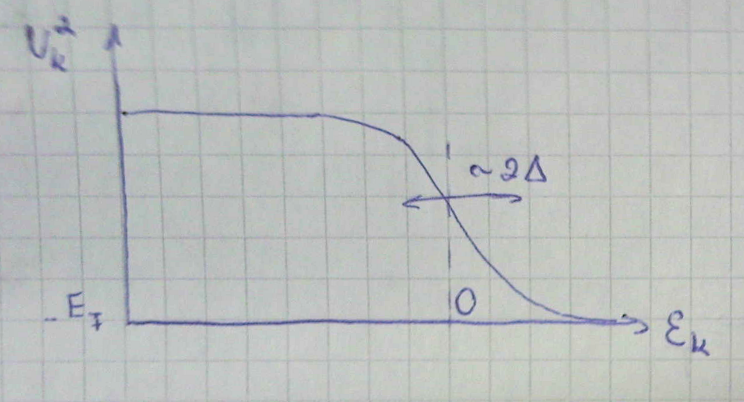
\includegraphics[width=0.45\textwidth]{kap13_15.png}


Kondensationsnergie 

\[W = -\frac{1}{2} D(E_F)\Delta^2\]

Quasiteilchen = ungepaarte Eletkronen und Löcher. Energie:

\[E_k = \sqrt{\epsilon^2_k+\Delta^2}\]

für Normalleiter: 

\[E_k = \epsilon_k = \frac{\hbar k^2}{2m}\]


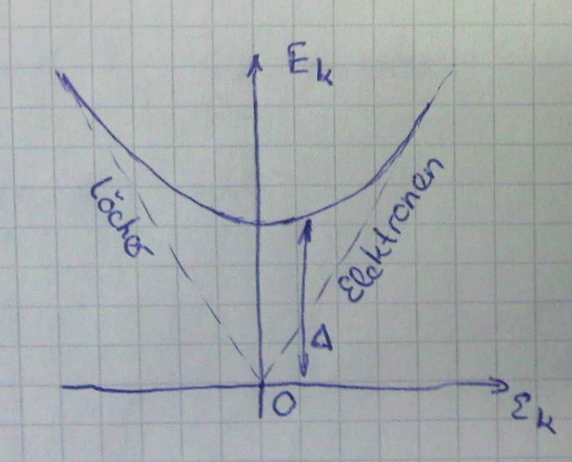
\includegraphics[width=0.45\textwidth]{kap13_16.png}



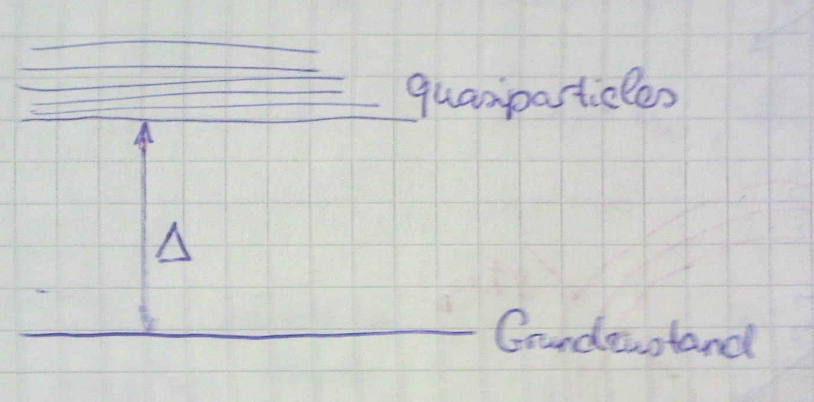
\includegraphics[width=0.45\textwidth]{kap13_17.png}


Kohärenzlänge:

\[\xi_0 \approx \Delta x \approx \frac{\hbar}{p}\approx \frac{1}{\Delta k}\]

\[\Delta k \approx \frac{2\Delta\cdot k_F}{E_F}\approx \frac{2\Delta\cdot 2m}{\hbar^2 k_F} = \frac{4\Delta}{\hbar^2 v_F}\]

\(\xi_0\approx 10 \text{ bis } 100nm\)

\subsection{Supraleiter 2.Art}

\(\rightarrow \) Flusschläuche = Flusswirbel = Vortices



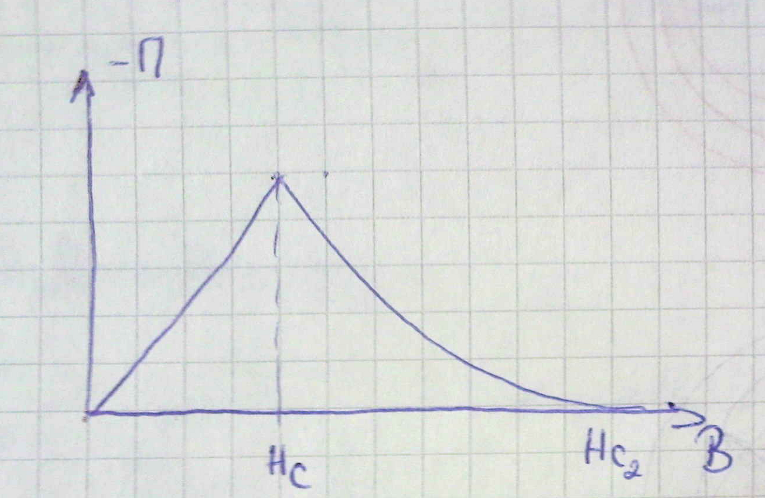
\includegraphics[width=0.45\textwidth]{kap13_18.png}


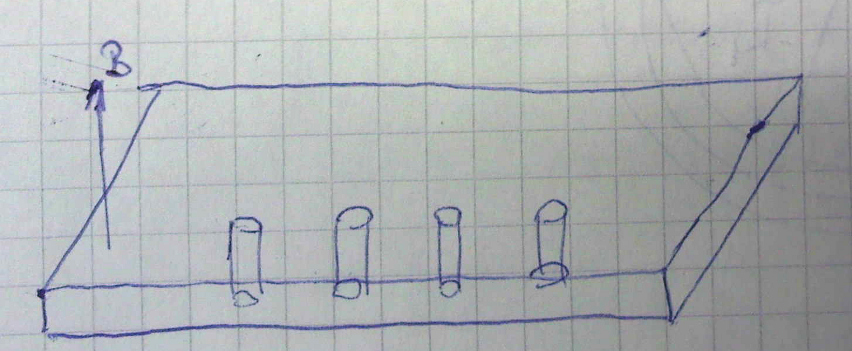
\includegraphics[width=0.45\textwidth]{kap13_19.png}


\(\lambda_L >> \xi_0  \rightarrow \) Supraleiter 2.Art

 \(\lambda_L < \xi_0  \rightarrow \) Supraleiter 1.Art


Theoretische Arbeit von Abrikosov vorschlagg dass die Vortices eine quadratische Struktur annehmen. Experiment von Essmann + Träuble (1967) ergab eine Hexagonale ('ähnlich' quadratisch) Struktur.

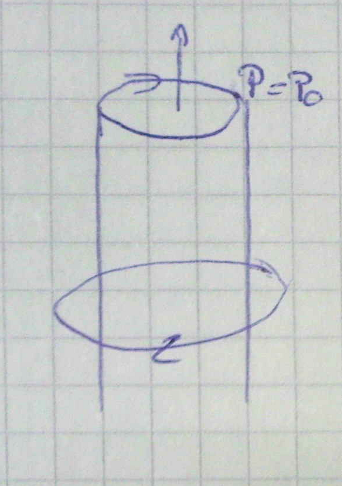
\includegraphics[width=0.25\textwidth]{kap13_20.png}

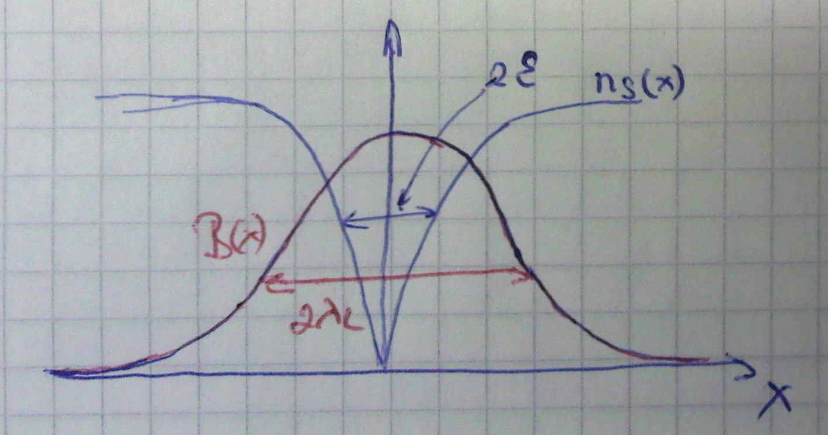
\includegraphics[width=0.45\textwidth]{kap13_21.png}


\end{document}
